% =============================================================================
%  Software Switch – Project Documentation
%  PSIP Semester Project  |  2025/2026
% =============================================================================
\documentclass[12pt,a4paper]{article}

% --- Encoding & language ---
\usepackage[utf8]{inputenc}
\usepackage[T1]{fontenc}
\usepackage[english]{babel}

% --- Page layout ---
\usepackage[top=2.5cm, bottom=2.5cm, left=2.5cm, right=2.5cm]{geometry}

% --- Typography ---
\usepackage[expansion=false]{microtype}
\usepackage{parskip}
\setlength{\parindent}{0pt}

% --- Math & symbols ---
\usepackage{amsmath}

% --- Tables ---
\usepackage{booktabs}
\usepackage{tabularx}
\usepackage{longtable}
\usepackage{array}
\usepackage{multirow}

% --- Graphics & colours ---
\usepackage{graphicx}
\usepackage{xcolor}
\definecolor{codebg}{RGB}{245,245,245}
\definecolor{linkblue}{RGB}{0,70,160}

% --- TikZ diagrams ---
\usepackage{tikz}
\usetikzlibrary{arrows.meta, positioning, shapes.geometric,
                decorations.pathreplacing, fit, backgrounds, calc}

% Shared node styles
\tikzset{
  sbox/.style  = {rectangle, draw, rounded corners=3pt, align=center,
                  font=\small, inner sep=5pt,
                  minimum width=3.6cm, minimum height=0.85cm},
  bluebox/.style  = {sbox, fill=blue!10,  draw=blue!50!black},
  greenbox/.style = {sbox, fill=green!10, draw=green!50!black},
  redbox/.style   = {sbox, fill=red!8,    draw=red!50!black},
  graybox/.style  = {sbox, fill=gray!10,  draw=gray!50},
  orangebox/.style= {sbox, fill=orange!12,draw=orange!60!black},
  diam/.style  = {diamond, draw, fill=yellow!15, align=center, font=\small,
                  inner sep=3pt, aspect=2.4,
                  minimum width=3.2cm, minimum height=1.1cm},
  arr/.style   = {-{Stealth[length=5pt]}, thick},
  darr/.style  = {{Stealth[length=5pt]}-{Stealth[length=5pt]}, thick},
  lbl/.style   = {font=\tiny, inner sep=1pt},
}

% --- Hyperlinks ---
\usepackage[colorlinks=true, linkcolor=linkblue, urlcolor=linkblue,
            citecolor=linkblue, pdfborder={0 0 0}]{hyperref}

% --- Headers / footers ---
\usepackage{fancyhdr}
\setlength{\headheight}{14pt}
\pagestyle{fancy}
\fancyhf{}
\lhead{\small Software Switch -- Project Documentation}
\rhead{\small PSIP 2025/2026}
\cfoot{\thepage}
\renewcommand{\headrulewidth}{0.4pt}

% --- Caption styling ---
\usepackage{caption}
\captionsetup{font=small, labelfont=bf}

% --- Utilities ---
\usepackage{enumitem}
\usepackage{float}

% =============================================================================
\begin{document}
% =============================================================================

% ------------- Title page ----------------------------------------------------
\begin{titlepage}
  \centering
  \vspace*{2cm}
  {\LARGE\bfseries Software Switch\par}
  \vspace{0.5em}
  {\large Project Documentation\par}
  \vspace{3cm}
  {\large PSIP Semester Project\par}
  \vspace{0.5em}
  {\normalsize 2025/2026\par}
  \vfill
  {\small
    \textit{Note on AI tool usage:}
    Parts of the source code were generated and refined with the assistance of
    GitHub Copilot (an AI coding assistant).
    All generated content was reviewed and verified by the authors.
    \par
  }
\end{titlepage}

% ------------- Table of contents ---------------------------------------------
\tableofcontents
\clearpage

% =============================================================================
\section{Introduction}
% =============================================================================

This document describes the design and implementation plan for a two-port
\textbf{software Ethernet switch} as part of the PSIP semester project.

The switch operates at \emph{OSI Layer~2} (Data Link layer).  It captures raw
Ethernet frames on two network interfaces, learns source MAC addresses, applies
configurable traffic filters, forwards frames to the correct output port, and
tracks per-port traffic statistics.

\subsection{Implementation environment}

\begin{itemize}[noitemsep]
  \item \textbf{Language:} C\# (.NET~8)
  \item \textbf{Packet capture:} SharpPcap~6.3.1~\cite{sharppcap} -- backed by
    libpcap (Linux/macOS) or Npcap (Windows)
  \item \textbf{Web interface:} built-in \texttt{HttpListener} (no external web
    framework)
  \item \textbf{Unit testing:} xUnit
\end{itemize}

SharpPcap provides cross-platform access to raw network interfaces in
promiscuous mode, enabling the switch to capture all frames regardless of their
destination MAC.

\subsection{Scope}

\begin{enumerate}[noitemsep]
  \item Frame reception, processing, and forwarding (Section~\ref{sec:forwarding})
  \item MAC address table management (Section~\ref{sec:mac})
  \item Traffic filtering (Section~\ref{sec:filtering})
  \item Traffic statistics (Section~\ref{sec:stats})
  \item Cable disconnection and replacement (Section~\ref{sec:cable})
  \item Optional protocol extensions: Syslog, CDP, RESTCONF
        (Section~\ref{sec:extensions})
\end{enumerate}

% =============================================================================
\section{System Architecture}
% =============================================================================

\subsection{Component overview}

The system consists of four cooperating components, arranged in a layered
architecture:

\begin{center}
\begin{tabular}{cp{9.5cm}}
\toprule
\textbf{Layer} & \textbf{Component} \\
\midrule
5 (top) & \textbf{Web GUI} (\texttt{HttpListener}) -- administrator interface for bridge
          start/stop, MAC table inspection, statistics display, and ACL management. \\
4       & \textbf{MAC Table} (+ TTL expiry task) \quad\textbar\quad \textbf{Port Statistics} (+ ACL rules)
          -- data stores queried by the GUI and updated by the core. \\
3       & \textbf{Switch Core} -- MAC learning, ACL filtering, forwarding decision,
          statistics update.  Receives frames from layer~2 and sends them back down. \\
2       & \textbf{SharpPcap capture layer} -- opens both NICs in promiscuous mode
          with \texttt{NoCaptureLocal}; delivers raw frames to the core via
          \texttt{OnPacketArrival} callbacks. \\
1 (bottom) & \textbf{NIC\,/\,Port~1} \quad\textbar\quad \textbf{NIC\,/\,Port~2}
              -- physical (or virtual) network interfaces. \\
\bottomrule
\end{tabular}
\end{center}

Data flows \emph{upward} from the NICs through the capture layer into the
switch core, and \emph{downward} when the core forwards a frame to the
opposite port.  The Web GUI reads MAC table and statistics data from layers~4.

\subsection{Thread and task model}

\begin{description}[noitemsep]
  \item[Capture callbacks] SharpPcap dispatches \texttt{OnPacketArrival} events
    from its internal per-device background threads (one per port).  Both
    callbacks share a single \texttt{lock} before touching the MAC table or
    statistics.
  \item[MAC expiry task] A background \texttt{async Task} wakes every 5~seconds
    and removes entries whose age exceeds the configured TTL.
  \item[Web server thread] The \texttt{HttpListener} thread handles HTTP
    requests from the administrator's browser.
\end{description}

% =============================================================================
\section{Frame Reception, Processing, and Forwarding}
\label{sec:forwarding}
% =============================================================================

\subsection{Ethernet~II frame structure}

The switch operates exclusively on \emph{Ethernet~II} frames
(IEEE~802.3~\cite{ieee8023} with EtherType $\geq$ 0x0600).

\begin{center}
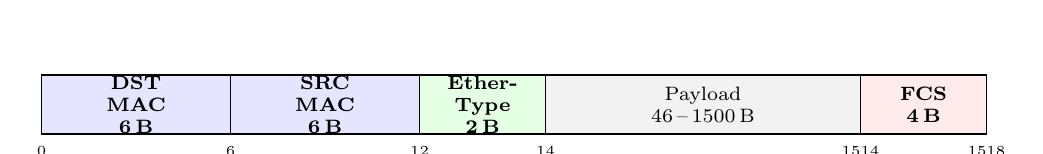
\begin{tikzpicture}[x=1cm, y=0.75cm]
  \draw[fill=blue!10]  (0,0) rectangle (2.4,1)
    node[midway, align=center, font=\scriptsize\bfseries] {DST\\MAC\\6\,B};
  \draw[fill=blue!10]  (2.4,0) rectangle (4.8,1)
    node[midway, align=center, font=\scriptsize\bfseries] {SRC\\MAC\\6\,B};
  \draw[fill=green!10] (4.8,0) rectangle (6.4,1)
    node[midway, align=center, font=\scriptsize\bfseries] {Ether-\\Type\\2\,B};
  \draw[fill=gray!10]  (6.4,0) rectangle (10.4,1)
    node[midway, align=center, font=\scriptsize] {Payload\\46\,--\,1500\,B};
  \draw[fill=red!8]   (10.4,0) rectangle (12,1)
    node[midway, align=center, font=\scriptsize\bfseries] {FCS\\4\,B};
  \foreach \x/\lb in {0/0, 2.4/6, 4.8/12, 6.4/14, 10.4/1514, 12/1518}
    \node[font=\tiny, below=1pt] at (\x,0) {\lb};
\end{tikzpicture}
\end{center}

Bytes~0--5 carry the destination MAC; bytes~6--11 carry the source MAC.
The EtherType field (bytes~12--13) identifies the upper-layer protocol.
Key EtherType values used in this project:

\begin{center}
\begin{tabular}{ll}
\toprule
\textbf{EtherType} & \textbf{Protocol} \\
\midrule
0x0800 & IPv4 \\
0x0806 & ARP \\
0x86DD & IPv6 \\
0x8100 & 802.1Q VLAN tag \\
\bottomrule
\end{tabular}
\end{center}

\subsection{Frame forwarding pipeline}

The complete per-frame processing pipeline is described below.
The three types of destination address receive distinct treatment:

\begin{itemize}[noitemsep]
  \item \textbf{BROADCAST} -- destination FF:FF:FF:FF:FF:FF.  The frame is
    flooded to the opposite port.
  \item \textbf{UNKNOWN UNICAST} -- unicast destination not yet in the MAC
    table.  The frame is flooded to the opposite port (standard behaviour).
  \item \textbf{KNOWN UNICAST} -- destination found in the MAC table.  The
    frame is forwarded to the learned port.
\end{itemize}

In all cases, IN-direction filters are checked first; OUT-direction filters are
checked before the frame is actually transmitted.

The complete frame processing pipeline is described step by step below.
Each step follows directly from the previous one; branching points are
indicated explicitly.

\begin{enumerate}
  \item \textbf{Frame received on port $P_{\mathrm{in}}$.}

  \item \textbf{Length check:} Is the frame at least 14~bytes long?
    \begin{itemize}[noitemsep]
      \item \emph{No} $\to$ \textbf{Discard} (frame too short). Processing
            stops.
      \item \emph{Yes} $\to$ continue.
    \end{itemize}

  \item \textbf{IN ACL filter} for port $P_{\mathrm{in}}$, direction~IN.
    \begin{itemize}[noitemsep]
      \item \emph{Deny} $\to$ \textbf{Discard} (ACL IN deny). Processing
            stops.
      \item \emph{Permit} $\to$ continue.
    \end{itemize}

  \item \textbf{Parse} destination MAC (bytes~0--5) and source MAC
        (bytes~6--11).

  \item \textbf{MAC learning:} record SRC~MAC $\mapsto P_{\mathrm{in}}$ in the
        MAC table and reset the TTL timer.

  \item \textbf{Forwarding decision -- determine $P_{\mathrm{out}}$:}
    \begin{itemize}[noitemsep]
      \item If DST~MAC is \texttt{FF:FF:FF:FF:FF:FF} $\to$
            \textbf{BROADCAST}: set $P_{\mathrm{out}}$ = opposite port.
      \item Else if DST~MAC is \emph{not} in the MAC table $\to$
            \textbf{UNKNOWN UNICAST}: set $P_{\mathrm{out}}$ = opposite port
            (flood).
      \item Else (DST~MAC found in table) $\to$
            \textbf{KNOWN UNICAST}: set $P_{\mathrm{out}}$ = table lookup
            result.
    \end{itemize}

  \item \textbf{Same-port guard:} If $P_{\mathrm{out}} = P_{\mathrm{in}}$,
        override $P_{\mathrm{out}}$ to the opposite port (prevents the
        frame from being sent back on the port it arrived on).

  \item \textbf{OUT ACL filter} for port $P_{\mathrm{out}}$, direction~OUT.
    \begin{itemize}[noitemsep]
      \item \emph{Deny} $\to$ \textbf{Discard} (ACL OUT deny). Processing
            stops.
      \item \emph{Permit} $\to$ continue.
    \end{itemize}

  \item \textbf{Update statistics:} increment RX counters on
        $P_{\mathrm{in}}$ and TX counters on $P_{\mathrm{out}}$ (both
        frame count and per-protocol PDU counters).

  \item \textbf{Transmit} the frame on port $P_{\mathrm{out}}$.
\end{enumerate}

\subsubsection{Processing order rationale}

\begin{enumerate}[noitemsep]
  \item \textbf{IN ACL first} -- A frame that violates an inbound rule is
    discarded immediately, before any MAC learning or table lookup, preventing
    learning of spoofed source addresses.
  \item \textbf{MAC learning before forwarding} -- The source MAC is recorded
    even if the destination is ultimately filtered by the OUT ACL.
  \item \textbf{OUT ACL before transmit} -- Allows per-port egress policies
    independently of ingress policies.
  \item \textbf{Statistics after OUT ACL} -- Counters reflect only frames that
    are actually transmitted (dropped frames are not counted as TX).
  \item \textbf{Promiscuous mode} -- Both pcap devices are opened with
    \texttt{DeviceModes.Promiscuous} so all frames on the medium are captured.
  \item \textbf{NoCaptureLocal} -- Prevents the capture device from seeing
    frames that the bridge itself injected, eliminating forwarding loops.
\end{enumerate}

\subsection{Protocol classification}
\label{sec:detection}

After extracting MACs, the switch inspects EtherType and higher-layer headers
to classify the frame for statistics purposes.  Detection is hierarchical: an
HTTP frame also increments TCP, IP, and Ethernet~II counters.

\begin{table}[H]
\centering
\caption{Protocol detection logic.}
\label{tab:protos}
\begin{tabularx}{\linewidth}{llX}
\toprule
\textbf{Protocol} & \textbf{Detection condition} & \textbf{Notes} \\
\midrule
Ethernet~II & always & Base layer; every frame is counted. \\
ARP         & EtherType = 0x0806 & Address Resolution Protocol. \\
IP          & EtherType = 0x0800, frame $\geq$ 34\,B & IPv4 only. \\
ICMP        & IP proto = 1 & Echo / ping traffic. \\
TCP         & IP proto = 6, frame $\geq$ l4start+20\,B & \\
HTTP        & TCP port\,80, payload starts with HTTP verb or \texttt{HTTP/} &
              Plaintext HTTP only. \\
UDP         & IP proto = 17 & \\
\bottomrule
\end{tabularx}
\end{table}

% =============================================================================
\section{MAC Address Table Management}
\label{sec:mac}
% =============================================================================

\subsection{Data structure}

The MAC table is an in-memory dictionary keyed on the colon-separated
17-character MAC string (e.g.\ \texttt{aa:bb:cc:dd:ee:ff}).
Each entry stores:

\begin{center}
\begin{tabular}{lll}
\toprule
\textbf{Field}    & \textbf{Type}     & \textbf{Meaning} \\
\midrule
\texttt{Port}     & \texttt{int}      & Port (1 or 2) where the host was last seen. \\
\texttt{LastSeen} & \texttt{DateTime} & UTC timestamp of the last frame from this MAC. \\
\bottomrule
\end{tabular}
\end{center}

Thread safety is ensured via a shared lock object acquired by the capture
callbacks, the expiry task, and any Web GUI read operations.

\subsection{Adding and updating entries (MAC learning)}

Every processed frame causes the \emph{source} MAC to be examined:

\begin{itemize}[noitemsep]
  \item If the MAC is \textbf{not} in the table, a new entry is created with
    the current port and the current UTC timestamp.
  \item If the MAC \textbf{is} already present but on a different port (port
    migration scenario), the existing entry's port and timestamp are updated
    in place atomically inside the lock.
  \item If the MAC is already present on the same port, only the timestamp
    is refreshed (TTL reset).
\end{itemize}

MAC learning is a side-effect of forwarding; no separate ``add'' API is
exposed.  This in-place update means the switch converges to the new topology
within a single frame after a cable swap (see Section~\ref{sec:cable}).

\subsection{Removing entries (TTL expiry)}

Each entry has a configurable time-to-live (default: \textbf{300\,s}).
A background task wakes every 5~seconds and removes entries whose age
$= \text{now} - \texttt{LastSeen}$ exceeds the TTL.

The TTL can be changed at runtime via the web GUI or the \texttt{SetMacTtl()}
API without restarting the switch.  Entries can also be cleared immediately
with the ``Clear MAC table'' button, which calls \texttt{ClearMacTable()} under
the lock.

% =============================================================================
\section{Traffic Filtering}
\label{sec:filtering}
% =============================================================================

\subsection{ACL model with IN/OUT directions}

Each port has two independent ACL (Access Control List) rule lists:
\textbf{IN-direction} (applied to arriving frames) and
\textbf{OUT-direction} (applied before transmitting frames).
This is analogous to Cisco IOS interface ACLs.

The following describes where each filter list is applied in the
processing pipeline.

The ACL filter pipeline operates as follows:

\begin{enumerate}[noitemsep]
  \item Frame arrives on port $P_{\mathrm{in}}$.
  \item \textbf{IN ACL} (port $P_{\mathrm{in}}$, direction~IN):
        rules are evaluated in priority order.
        If a \emph{deny} rule matches $\to$ frame is dropped and logged;
        processing stops.
        If all rules permit (or no matching rule exists) $\to$ continue.
  \item MAC learning + forwarding decision (determine $P_{\mathrm{out}}$).
  \item \textbf{OUT ACL} (port $P_{\mathrm{out}}$, direction~OUT):
        rules are evaluated in priority order.
        If a \emph{deny} rule matches $\to$ frame is dropped and logged;
        processing stops.
        If all rules permit $\to$ continue.
  \item Transmit on $P_{\mathrm{out}}$.
\end{enumerate}

\subsection{Rule structure}

Each rule is evaluated in priority order and specifies the following fields:

\begin{center}
\begin{tabular}{lll}
\toprule
\textbf{Field}   & \textbf{Example}                   & \textbf{Notes} \\
\midrule
Priority         & 10, 20, 30, \ldots                 & Lower = higher priority. \\
Direction        & IN, OUT                            & Per-port direction. \\
Match: src MAC   & \texttt{aa:bb:cc:dd:ee:ff} / any   & Exact or wildcard. \\
Match: dst MAC   & broadcast, multicast group          & \\
Match: EtherType & 0x0800 (IP), 0x0806 (ARP)           & \\
Match: in-port   & 1, 2, any                           & Only meaningful for IN rules. \\
Action           & permit / deny                       & \\
\bottomrule
\end{tabular}
\end{center}

\subsection{Rule matching and specificity}

Rules are evaluated in ascending priority order (priority~10 before
priority~20).  The first rule whose match criteria are satisfied determines
the action.  If no rule matches, the default action is \textbf{permit}.

To handle varying specificity, the administrator assigns lower priority numbers
to more specific rules.  Example:

\begin{center}
\begin{tabular}{lllll}
\toprule
\textbf{Prio} & \textbf{Direction} & \textbf{Src MAC} & \textbf{EtherType} & \textbf{Action} \\
\midrule
10 & IN & \texttt{de:ad:be:ef:00:01} & any    & deny   \\
20 & IN & any                        & 0x0806 & permit \\
30 & IN & any                        & any    & permit \\
\bottomrule
\end{tabular}
\end{center}

Rule~10 blocks a specific MAC regardless of protocol; rule~20 explicitly allows
ARP from any other source; rule~30 permits everything else.

\subsection{Layer-3 / Layer-4 filtering extension}

Because the switch already classifies frames by protocol
(Section~\ref{sec:detection}), extended rules could additionally inspect:

\begin{itemize}[noitemsep]
  \item IPv4 source / destination address (bytes 26--29 / 30--33)
  \item TCP/UDP source and destination port numbers (bytes 34--35 / 36--37)
  \item ICMP type and code (bytes 34--35)
\end{itemize}

This is equivalent to a Cisco IOS \emph{extended ACL}, allowing fine-grained
layer-4 policies (e.g.\ block HTTP to a specific host, allow DNS only).

% =============================================================================
\section{Traffic Statistics}
\label{sec:stats}
% =============================================================================

\subsection{Counters maintained}

The switch maintains per-port RX and TX counters at two levels:

\begin{center}
\begin{tabular}{lll}
\toprule
\textbf{Counter}   & \textbf{Dir.} & \textbf{Description} \\
\midrule
\texttt{RxFrames}  & RX & Total Ethernet frames received on this port. \\
\texttt{TxFrames}  & TX & Total Ethernet frames transmitted on this port. \\
\texttt{RxPdus[p]} & RX & PDU count for protocol $p$ on receive. \\
\texttt{TxPdus[p]} & TX & PDU count for protocol $p$ on transmit. \\
\bottomrule
\end{tabular}
\end{center}

where $p \in \{\texttt{ethernet\_ii},\ \texttt{arp},\ \texttt{ip},\
\texttt{tcp},\ \texttt{udp},\ \texttt{icmp},\ \texttt{http}\}$.

Counters are incremented atomically inside the shared lock, preventing
race conditions between the two capture threads.

\subsection{Update logic}

Statistics are updated \emph{after} the OUT ACL check (only actually
transmitted frames are counted as TX):

\begin{itemize}[noitemsep]
  \item \texttt{RxFrames} and \texttt{RxPdus} are incremented for
    $P_{\mathrm{in}}$ after every frame that passes the IN ACL.
  \item \texttt{TxFrames} and \texttt{TxPdus} are incremented for
    $P_{\mathrm{out}}$ only if the frame also passes the OUT ACL.
\end{itemize}

Protocol counting is \emph{hierarchical}: an HTTP frame increments
\texttt{http}, \texttt{tcp}, \texttt{ip}, and \texttt{ethernet\_ii}
simultaneously.  A frame arriving on port~1 and forwarded to port~2 therefore
increments port~1 RX and port~2 TX.

The exact positions in the pipeline where each counter group is updated are:

\begin{enumerate}[noitemsep]
  \item Frame arrives on $P_{\mathrm{in}}$.
  \item IN ACL filter (if \emph{deny} $\to$ drop; no counters incremented).
  \item Protocol detection (identify Ethernet~II, ARP, IP, ICMP, TCP, UDP, HTTP).
  \item \textbf{Increment $P_{\mathrm{in}}$\texttt{.RxFrames}} and
        \texttt{RxPdus[\ldots]} for each detected protocol layer.
  \item Forwarding decision (choose $P_{\mathrm{out}}$).
  \item OUT ACL filter (if \emph{deny} $\to$ drop; TX counters
        \emph{not} incremented).
  \item \textbf{Increment $P_{\mathrm{out}}$\texttt{.TxFrames}} and
        \texttt{TxPdus[\ldots]} for each detected protocol layer.
  \item Transmit on $P_{\mathrm{out}}$.
\end{enumerate}

% =============================================================================
\section{Cable Disconnection and Replacement}
\label{sec:cable}
% =============================================================================

\subsection{Cable removal -- detection mechanism}

When a network cable is physically unplugged, the network interface card (NIC)
detects the loss of the link signal and transitions to the
\emph{link-down} state.  The operating system updates the interface's
operational status accordingly.

\subsubsection{SharpPcap exception-based detection}

SharpPcap surfaces link-down events as a \texttt{PcapException} thrown on the
capture device.  When the exception is caught, the switch takes the following
steps:

\begin{enumerate}[noitemsep]
  \item Log a warning indicating which port lost its link.
  \item Immediately flush all MAC table entries last seen on the affected port
    (calling \texttt{FlushEntriesForPort(port)}).
  \item Attempt to reopen the capture device with an exponential back-off retry
    (e.g.\ 1~s, 2~s, 4~s) to detect cable re-insertion automatically.
\end{enumerate}

\subsubsection{NetworkChange-based detection}

An alternative approach uses the .NET \texttt{NetworkChange.NetworkAddress\-Changed}
event, which fires whenever any network interface changes its address or
operational status.  On link-down, the handler iterates over all interfaces and
flushes the MAC table for any port mapped to an interface with
\texttt{OperationalStatus.Down}.  This approach works even when the pcap device
does not raise an exception (e.g.\ on Windows with Npcap).

\subsubsection{Scenario: cable pulled on port $N$}

\begin{enumerate}[noitemsep]
  \item Link-down detected (exception or NetworkChange event).
  \item MAC entries for port~$N$ are flushed immediately.
  \item Subsequent frames addressed to hosts that were on port~$N$ are now
    treated as unknown unicast and flooded to the opposite port.
  \item If the link never comes back, no further entries accumulate for port~$N$.
\end{enumerate}

\textbf{Fallback -- TTL-based passive expiry:}  If neither detection mechanism
is available, the switch falls back to passive TTL expiry.  Entries last seen on
port~$N$ survive until their TTL expires (default 300~s); during this window,
frames toward those hosts are forwarded to a link-down interface and silently
dropped by the OS.

\subsection{Cable replacement (port migration)}

When a host moves from one port to another (or the same cable is plugged back
in), the switch must update its MAC table to reflect the new topology.
The in-place update in MAC learning (Section~\ref{sec:mac}) handles this:

\begin{enumerate}[noitemsep]
  \item The host sends its first frame on the new port.
  \item The switch sees the source MAC arriving on a different port than
    recorded and updates the entry (port + timestamp) atomically.
  \item Convergence is complete after \emph{one frame} -- no flooding or
    spanning-tree recalculation is required.
\end{enumerate}

The convergence timeline after a cable swap is:

\begin{description}[noitemsep]
  \item[$t_0$:] Host~A is connected to Port~1.  MAC table contains:
        A~$\to$~Port~1.
  \item[$t_1$:] Cable is physically moved from Port~1 to Port~2.
    \begin{enumerate}[noitemsep]
      \item Link-down detected on Port~1 $\Rightarrow$ all MAC entries for
            Port~1 are flushed immediately.
      \item First frame from Host~A arrives on Port~2.
      \item MAC table is updated: A~$\to$~Port~2.
    \end{enumerate}
  \item[$t_2$:] Switch has converged (after \emph{one frame}).
\end{description}

\subsection{Edge-case summary}

\begin{center}
\begin{tabular}{p{3.4cm}p{5.4cm}p{4.4cm}}
\toprule
\textbf{Event} & \textbf{Behaviour} & \textbf{Detection method} \\
\midrule
Cable pulled (link down) &
  MAC entries for the port flushed immediately. &
  PcapException or NetworkChange event. \\
Cable re-inserted, same host &
  Entry refreshed on first frame after link-up. &
  No action needed. \\
Host moved to other port &
  Entry updated on first frame from new port (one-frame convergence). &
  Implicit via MAC learning. \\
Both cables pulled &
  Both port tables flushed; switch idles. &
  Two link-down events. \\
\bottomrule
\end{tabular}
\end{center}

% =============================================================================
\section{Optional Extensions: Syslog, CDP, RESTCONF}
\label{sec:extensions}
% =============================================================================

The following protocols are analysed below as potential extensions.  Each
analysis covers the purpose of the protocol, its packet/frame structure with
field-level detail, and how the switch would use it.

% -----------------------------------------------------------------------------
\subsection{Syslog (RFC~5424)}
% -----------------------------------------------------------------------------

\subsubsection{Purpose}

Syslog provides a standard mechanism for forwarding log messages to a central
collector~\cite{rfc5424}.  The switch would emit Syslog messages for events
such as: new MAC address learned, MAC migrated to new port, MAC entry expired,
frame discarded by ACL filter, and link-down detected.

\subsubsection{Network encapsulation}

A Syslog message is transported inside a \textbf{UDP datagram} (RFC~5424
default; TCP on port~6514 is used for reliable delivery).  The encapsulation
stack is:

\begin{center}
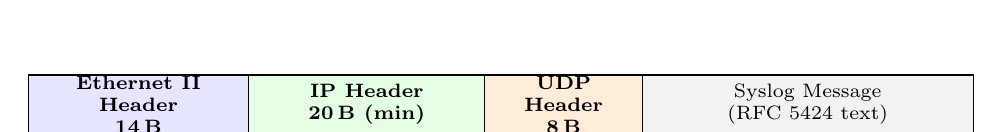
\begin{tikzpicture}[x=1.0cm, y=0.75cm]
  \draw[fill=blue!10]  (0,0) rectangle (2.8,1)
    node[midway, align=center, font=\scriptsize\bfseries]
    {Ethernet~II\\Header\\14\,B};
  \draw[fill=green!10] (2.8,0) rectangle (5.8,1)
    node[midway, align=center, font=\scriptsize\bfseries]
    {IP Header\\20\,B (min)};
  \draw[fill=orange!15](5.8,0) rectangle (7.8,1)
    node[midway, align=center, font=\scriptsize\bfseries]
    {UDP\\Header\\8\,B};
  \draw[fill=gray!10]  (7.8,0) rectangle (12.0,1)
    node[midway, align=center, font=\scriptsize]
    {Syslog Message\\(RFC~5424 text)};
\end{tikzpicture}
\end{center}

\paragraph{Ethernet~II header fields (switch $\to$ collector):}
\begin{center}
\begin{tabular}{lll}
\toprule
\textbf{Field} & \textbf{Value} & \textbf{Notes} \\
\midrule
DST MAC      & collector MAC address & Resolved via ARP. \\
SRC MAC      & switch management MAC & \\
EtherType    & \texttt{0x0800} & IPv4. \\
\bottomrule
\end{tabular}
\end{center}

\paragraph{IPv4 header fields:}
\begin{center}
\begin{tabular}{lll}
\toprule
\textbf{Field} & \textbf{Value} & \textbf{Notes} \\
\midrule
Version      & 4            & IPv4. \\
IHL          & 5 (20\,B)    & No options. \\
DSCP/ECN     & 0            & Best effort. \\
TTL          & 64           & Standard default. \\
Protocol     & 17 (0x11)    & UDP. \\
SRC IP       & switch management IP & \\
DST IP       & syslog collector IP & \\
\bottomrule
\end{tabular}
\end{center}

\paragraph{UDP header fields:}
\begin{center}
\begin{tabular}{lll}
\toprule
\textbf{Field} & \textbf{Value} & \textbf{Notes} \\
\midrule
Source port  & ephemeral (e.g.\ 49152--65535) & OS-assigned. \\
Dest.\ port  & \textbf{514}   & Standard Syslog port (UDP). \\
Length       & 8 + payload    & \\
Checksum     & computed       & \\
\bottomrule
\end{tabular}
\end{center}

\subsubsection{RFC~5424 message format}

An RFC~5424 Syslog message consists of a HEADER and an optional
STRUCTURED-DATA block followed by the free-text MSG:

\begin{center}
\texttt{<PRI>VERSION SP TIMESTAMP SP HOSTNAME SP APP-NAME SP PROCID SP MSGID
SP [STRUCTURED-DATA] SP MSG}
\end{center}

\paragraph{Priority (PRI) field:}
$\texttt{PRI} = (\mathrm{Facility} \times 8) + \mathrm{Severity}$.
Example: Local~0 (facility~16), Informational (severity~6)
$\Rightarrow \texttt{<134>}$.

\begin{center}
\begin{tabular}{lll}
\toprule
\textbf{Facility} & \textbf{Code} & \textbf{Used for} \\
\midrule
kern      & 0  & Kernel messages. \\
user      & 1  & User-level messages. \\
local0--7 & 16--23 & Locally defined; \textbf{local0 (16)} used by the switch. \\
\bottomrule
\end{tabular}
\end{center}

\begin{center}
\begin{tabular}{lll}
\toprule
\textbf{Severity} & \textbf{Code} & \textbf{Switch usage} \\
\midrule
Emergency  & 0 & System unusable. \\
Alert      & 1 & \\
Critical   & 2 & Link-down detected. \\
Error      & 3 & Capture device failure. \\
Warning    & 4 & Frame discarded by ACL filter. \\
Notice     & 5 & MAC migrated to new port. \\
Info       & 6 & New MAC address learned. \\
Debug      & 7 & MAC entry expired (TTL). \\
\bottomrule
\end{tabular}
\end{center}

\paragraph{STRUCTURED-DATA example (RFC~5424 format):}

\texttt{[switch@12345 port="1" mac="aa:bb:cc:dd:ee:ff" event="learned"]}

\paragraph{Complete example message:}

The \textbf{Software Switch} (syslog sender) sends a
UDP datagram to port~514 of the \textbf{Syslog Collector}:

\begin{center}
\small\texttt{<134>1 2026-03-10T12:00:00.000Z sw-01 switch - MACLEARN
[switch@12345 port="1" mac="aa:bb:cc:dd:ee:ff"] New MAC address learned}
\end{center}

% -----------------------------------------------------------------------------
\subsection{CDP -- Cisco Discovery Protocol}
% -----------------------------------------------------------------------------

\subsubsection{Purpose}

CDP~\cite{cdp} is a Cisco proprietary Layer-2 protocol.  Cisco devices
periodically advertise their identity and capabilities to directly connected
neighbours.  The software switch could passively decode CDP frames to identify
the types of devices connected to each port, logging device ID, platform, and
IP address without participating in the CDP domain.

\subsubsection{Frame encapsulation}

CDP is \textbf{not} encapsulated in Ethernet~II; it uses
\textbf{IEEE~802.3} with LLC/SNAP encapsulation:

\begin{center}
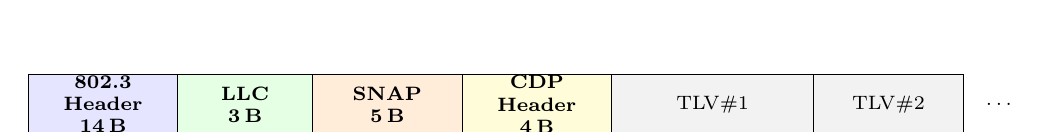
\begin{tikzpicture}[x=0.95cm, y=0.75cm]
  \draw[fill=blue!10]  (0,0) rectangle (2.0,1)
    node[midway,align=center,font=\scriptsize\bfseries] {802.3\\Header\\14\,B};
  \draw[fill=green!10] (2.0,0) rectangle (3.8,1)
    node[midway,align=center,font=\scriptsize\bfseries] {LLC\\3\,B};
  \draw[fill=orange!15](3.8,0) rectangle (5.8,1)
    node[midway,align=center,font=\scriptsize\bfseries] {SNAP\\5\,B};
  \draw[fill=yellow!15](5.8,0) rectangle (7.8,1)
    node[midway,align=center,font=\scriptsize\bfseries] {CDP\\Header\\4\,B};
  \draw[fill=gray!10]  (7.8,0) rectangle (10.5,1)
    node[midway,align=center,font=\scriptsize] {TLV\#1};
  \draw[fill=gray!10]  (10.5,0) rectangle (12.5,1)
    node[midway,align=center,font=\scriptsize] {TLV\#2};
  \node[font=\scriptsize] at (13.0, 0.5) {\ldots};
\end{tikzpicture}
\end{center}

\paragraph{802.3 Header fields (Cisco device $\to$ switch):}
\begin{center}
\begin{tabular}{lll}
\toprule
\textbf{Field}   & \textbf{Value}                        & \textbf{Notes} \\
\midrule
DST MAC          & \texttt{01:00:0C:CC:CC:CC}            & CDP multicast address. \\
SRC MAC          & sending interface MAC                  & \\
Length           & total frame size (excl.\ preamble/FCS) & $\leq$ 1500. \\
\bottomrule
\end{tabular}
\end{center}

\paragraph{LLC Header (3 bytes):}
\begin{center}
\begin{tabular}{lll}
\toprule
\textbf{Field}   & \textbf{Value} & \textbf{Notes} \\
\midrule
DSAP             & \texttt{0xAA}  & SNAP SAP identifier. \\
SSAP             & \texttt{0xAA}  & SNAP SAP identifier. \\
Control          & \texttt{0x03}  & Unnumbered frame (UI). \\
\bottomrule
\end{tabular}
\end{center}

\paragraph{SNAP Header (5 bytes):}
\begin{center}
\begin{tabular}{lll}
\toprule
\textbf{Field}   & \textbf{Value}         & \textbf{Notes} \\
\midrule
OUI              & \texttt{00:00:0C}      & Cisco OUI. \\
Protocol ID      & \texttt{0x2000}        & CDP protocol identifier. \\
\bottomrule
\end{tabular}
\end{center}

\paragraph{CDP Header (4 bytes):}
\begin{center}
\begin{tabular}{lll}
\toprule
\textbf{Field}   & \textbf{Value}   & \textbf{Notes} \\
\midrule
Version          & 1 or 2           & CDP version in use. \\
TTL              & 180              & Seconds until this advertisement expires. \\
Checksum         & computed         & 16-bit ones-complement checksum of entire CDP PDU. \\
\bottomrule
\end{tabular}
\end{center}

\subsubsection{TLV record structure}

Each CDP TLV (Type-Length-Value) record has the following fixed-size header
followed by a variable-length value:

\begin{center}
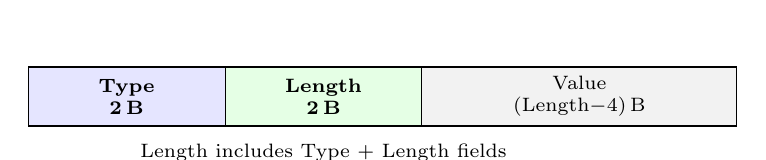
\begin{tikzpicture}[x=1.0cm, y=0.75cm]
  \draw[fill=blue!10]  (0,0) rectangle (2.5,1)
    node[midway,align=center,font=\scriptsize\bfseries] {Type\\2\,B};
  \draw[fill=green!10] (2.5,0) rectangle (5.0,1)
    node[midway,align=center,font=\scriptsize\bfseries] {Length\\2\,B};
  \draw[fill=gray!10]  (5.0,0) rectangle (9.0,1)
    node[midway,align=center,font=\scriptsize] {Value\\(Length$-$4)\,B};
  \node[font=\scriptsize, below=3pt] at (3.75,0) {Length includes Type + Length fields};
\end{tikzpicture}
\end{center}

\begin{center}
\begin{tabular}{lll}
\toprule
\textbf{Type} & \textbf{TLV Name}     & \textbf{Content / format} \\
\midrule
0x0001 & Device ID         & Hostname string (ASCII). \\
0x0002 & Addresses         & Count (4\,B) + address records; each: protocol type (1\,B),
                             length (1\,B), address bytes. \\
0x0003 & Port ID           & Interface name string (e.g.\ \texttt{GigabitEthernet0/1}). \\
0x0004 & Capabilities      & 4-byte bitmask (see Table~\ref{tab:cdpcap}). \\
0x0005 & Software Version  & Multi-line IOS version string. \\
0x0006 & Platform          & Hardware platform string (e.g.\ \texttt{cisco WS-C3560}). \\
0x0009 & VTP Mgmt Domain   & VTP domain name string. \\
0x000A & Native VLAN       & 2-byte VLAN ID. \\
0x000B & Duplex            & 1\,B: 0x00 = half, 0x01 = full. \\
0x000F & MTU               & 4-byte MTU value in bytes. \\
\bottomrule
\end{tabular}
\end{center}

\begin{table}[H]
\centering
\caption{CDP Capabilities bitmask (TLV type 0x0004).}
\label{tab:cdpcap}
\begin{tabular}{ll}
\toprule
\textbf{Bit} & \textbf{Capability} \\
\midrule
0x0001 & Router \\
0x0002 & Transparent bridge \\
0x0004 & Source-route bridge \\
0x0008 & Switch \\
0x0010 & Host \\
0x0020 & IGMP-capable \\
0x0040 & Repeater \\
\bottomrule
\end{tabular}
\end{table}

Figure~\ref{fig:cdp} shows the complete CDP frame structure.

\begin{figure}[H]
\centering
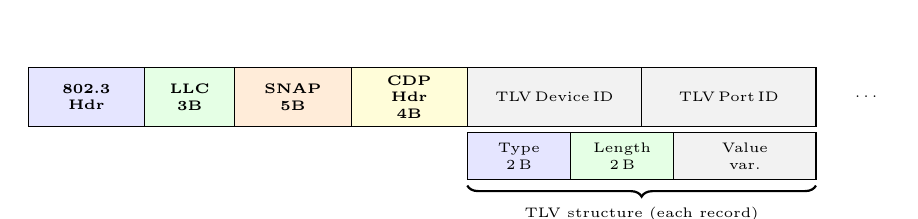
\begin{tikzpicture}[x=0.82cm, y=0.75cm]
  % Layer 1 - frame overview
  \draw[fill=blue!10]  (0,0) rectangle (1.8,1)
    node[midway,align=center,font=\tiny\bfseries] {802.3\\Hdr};
  \draw[fill=green!10] (1.8,0) rectangle (3.2,1)
    node[midway,align=center,font=\tiny\bfseries] {LLC\\3B};
  \draw[fill=orange!15](3.2,0) rectangle (5.0,1)
    node[midway,align=center,font=\tiny\bfseries] {SNAP\\5B};
  \draw[fill=yellow!15](5.0,0) rectangle (6.8,1)
    node[midway,align=center,font=\tiny\bfseries] {CDP\\Hdr\\4B};
  \draw[fill=gray!10]  (6.8,0) rectangle (9.5,1)
    node[midway,align=center,font=\tiny] {TLV\,Device\,ID};
  \draw[fill=gray!10]  (9.5,0) rectangle (12.2,1)
    node[midway,align=center,font=\tiny] {TLV\,Port\,ID};
  \node[font=\tiny] at (13.0, 0.5) {\ldots};

  % TLV breakdown
  \draw[fill=blue!10]  (6.8,-0.9) rectangle (8.4,-0.1)
    node[midway,align=center,font=\tiny] {Type\\2\,B};
  \draw[fill=green!10] (8.4,-0.9) rectangle (10.0,-0.1)
    node[midway,align=center,font=\tiny] {Length\\2\,B};
  \draw[fill=gray!10]  (10.0,-0.9) rectangle (12.2,-0.1)
    node[midway,align=center,font=\tiny] {Value\\var.};
  \draw[decorate,decoration={brace,amplitude=4pt,mirror},thick]
    (6.8,-1.0) -- (12.2,-1.0)
    node[midway,below=4pt,font=\tiny] {TLV structure (each record)};
\end{tikzpicture}
\caption{CDP 802.3/LLC/SNAP frame and TLV record structure.}
\label{fig:cdp}
\end{figure}

% -----------------------------------------------------------------------------
\subsection{RESTCONF (RFC~8040)}
% -----------------------------------------------------------------------------

\subsubsection{Purpose and scope}

RESTCONF~\cite{rfc8040} is a REST-based management protocol for YANG-modelled
network devices.  If implemented, it \emph{replaces} the current web GUI and
provides a standardised, machine-readable API for managing the switch.
RESTCONF also subsumes the need for custom filtering and CDP/Syslog integration
into the same management plane.

\subsubsection{Transport and security}

\begin{itemize}[noitemsep]
  \item \textbf{Transport:} HTTPS (TLS~1.2 or higher) -- mandatory per
    RFC~8040, §2.1.
  \item \textbf{Authentication:} HTTP Basic Auth (username / password over TLS)
    or token-based (HTTP Bearer token).
  \item \textbf{Content-Type:}
    \texttt{application/yang-data+json} (default) or
    \texttt{application/yang-data+xml}.
  \item \textbf{Port:} 443 (HTTPS) or a configurable management port (e.g.\
    8443).
\end{itemize}

\subsubsection{YANG model -- conceptual outline}

The following YANG containers would model the switch state:

\begin{center}
\begin{tabular}{lll}
\toprule
\textbf{YANG container}          & \textbf{Type}   & \textbf{Description} \\
\midrule
\texttt{switch:mac-table}         & list            & MAC entries (mac, port, last-seen, ttl-remaining). \\
\texttt{switch:mac-table/ttl}     & leaf (uint32)   & Global MAC TTL in seconds. \\
\texttt{switch:ports}             & list            & Port 1 and Port 2 configuration. \\
\texttt{switch:statistics}        & container       & Per-port RX/TX frame and PDU counters. \\
\texttt{switch:acl}               & list            & ACL rules (priority, direction, match, action). \\
\texttt{switch:acl/port/inbound}  & list            & IN-direction rules for a port. \\
\texttt{switch:acl/port/outbound} & list            & OUT-direction rules for a port. \\
\bottomrule
\end{tabular}
\end{center}

\subsubsection{REST API design}

\begin{center}
\begin{tabular}{p{1.2cm}p{6.5cm}p{5.0cm}}
\toprule
\textbf{Method} & \textbf{URL}                                           & \textbf{Action} \\
\midrule
GET    & \texttt{/restconf/data/switch:mac-table}               & Retrieve all MAC entries. \\
DELETE & \texttt{/restconf/data/switch:mac-table}               & Clear the MAC table. \\
PATCH  & \texttt{/restconf/data/switch:mac-table/ttl}           & Update MAC TTL. \\
GET    & \texttt{/restconf/data/switch:statistics}              & Retrieve port counters. \\
DELETE & \texttt{/restconf/data/switch:statistics}              & Reset counters. \\
GET    & \texttt{/restconf/data/switch:acl}                     & Retrieve all ACL rules. \\
POST   & \texttt{/restconf/data/switch:acl/port=1/inbound}      & Add IN rule for port~1. \\
DELETE & \texttt{/restconf/data/switch:acl/port=1/inbound/10}   & Delete rule priority~10. \\
GET    & \texttt{/restconf/data/switch:ports}                   & List ports and their status. \\
\bottomrule
\end{tabular}
\end{center}

\subsubsection{JSON message structure examples}

\paragraph{GET /restconf/data/switch:mac-table -- response body:}

\begin{verbatim}
{ "switch:mac-table": [
    { "mac": "aa:bb:cc:dd:ee:ff",
      "port": 1, "ttl-remaining": 245 },
    { "mac": "11:22:33:44:55:66",
      "port": 2, "ttl-remaining": 180 }
  ]
}
\end{verbatim}

\paragraph{PATCH /restconf/data/switch:mac-table/ttl -- request body:}

\begin{verbatim}
{ "switch:ttl": 600 }
\end{verbatim}

\paragraph{POST /restconf/data/switch:acl/port=1/inbound -- request body:}

\begin{verbatim}
{ "switch:rule": {
    "priority": 10,
    "src-mac": "de:ad:be:ef:00:01",
    "action": "deny" }
}
\end{verbatim}

\subsubsection{ARP and IP address handling}

The switch operates at Layer~2 and does not generate ARP requests itself.
If the RESTCONF server needs to send IP packets (e.g.\ Syslog or management
traffic), ARP resolution is handled transparently by the host operating system's
network stack, which manages the ARP cache and sends ARP requests on behalf of
any application that opens a socket.  This mechanism does not require any
explicit switch-level ARP implementation.

% =============================================================================
\section*{Conclusion}
\addcontentsline{toc}{section}{Conclusion}
% =============================================================================

The prototype demonstrates the essential functionality of an Ethernet Layer-2
switch: MAC learning with TTL expiry, BROADCAST / UNKNOWN UNICAST / KNOWN
UNICAST forwarding with both IN-direction and OUT-direction ACL filter support,
hierarchical protocol-aware statistics, and a web-based management interface.

Open items for a full production implementation include:

\begin{itemize}[noitemsep]
  \item Complete ACL rule engine with L3/L4 match support.
  \item Syslog integration (RFC~5424) for structured event logging.
  \item CDP passive decoding for neighbour discovery.
  \item RESTCONF / YANG API as a standardised management plane.
\end{itemize}

% =============================================================================
%  References
% =============================================================================
\begin{thebibliography}{9}

\bibitem{rfc5424}
R.~Gerhards,
\textit{The Syslog Protocol},
RFC~5424, IETF, March 2009.
\url{https://www.rfc-editor.org/rfc/rfc5424}

\bibitem{rfc8040}
A.~Bierman, M.~Bjorklund, K.~Watsen,
\textit{RESTCONF Protocol},
RFC~8040, IETF, January 2017.
\url{https://www.rfc-editor.org/rfc/rfc8040}

\bibitem{cdp}
Cisco Systems,
\textit{Cisco Discovery Protocol},
Cisco IOS documentation, 2024.
\url{https://www.cisco.com/c/en/us/td/docs/ios-xml/ios/cdp/configuration/15-mt/cdp-15-mt-book.html}

\bibitem{ieee8023}
IEEE,
\textit{IEEE Standard for Ethernet},
IEEE~802.3-2022.
\url{https://standards.ieee.org/ieee/802.3/10236/}

\bibitem{sharppcap}
C.~Morgan et al.,
\textit{SharpPcap -- A Packet Capture Framework for .NET},
GitHub, 2024.
\url{https://github.com/dotpcap/sharppcap}

\bibitem{wireshark}
Wireshark Foundation,
\textit{Wireshark Wiki -- Sample Captures}.
\url{https://wiki.wireshark.org/SampleCaptures}

\bibitem{netacad}
Cisco Networking Academy,
\textit{CCNA: Introduction to Networks -- Ethernet Switching},
NetAcad, 2023.
\url{https://www.netacad.com}

\bibitem{microsoftdotnet}
Microsoft,
\textit{.NET~8 -- NetworkChange, HttpListener, Task parallel library},
Microsoft Docs, 2024.
\url{https://learn.microsoft.com/en-us/dotnet/}

\end{thebibliography}

\end{document}
